	\section{تشخیص ارقام دست نویس}
	در بخش قبل با تجزیه مقادیر تکین آشنا شدیم. در این بخش 
	پس از بررسی داده و ارائه یک راه حل خوشه بندی\LTRfootnote{clustrering } به بررسی الگوریتم ارقام ویژه \LTRfootnote{eigen digits} می پردازیم. مروری کامل بر متود های مختلف در \cite{lecun} داده شده. 
	\subsection{پایگاه داده}
	در این مقاله از دیتاست MNIST \LTRfootnote{Modified National Institute of Standards and Technology} برای طبقه بندی ارقام دست نویس استفاده می کنیم.  
	این دیتاست شامل ۶۰۰۰۰ داده آموزش \LTRfootnote{train} و ۱۰۰۰۰ داده تست  \LTRfootnote{test} است. هر عکس در قالب یک آرایه ۲۸ در ۲۸ به ما داده شده. در مرحله پیش پردازش با صاف \LTRfootnote{flat} کردن عکس ها آنها را به صورت یک بردار با بعد ۷۸۴ نمایش می دهیم.\\
	هدف ما استفاده از داده های آموزشی برا طبقه بندی داده های تست است.
	 	 
	\begin{figure}[h]
		\centering
		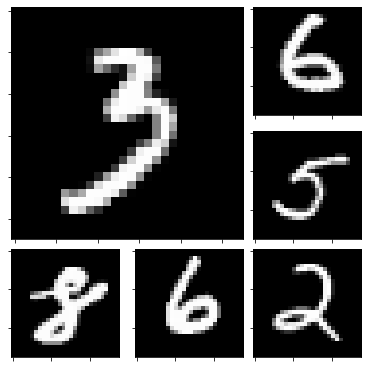
\includegraphics[width=0.7\linewidth]{assets/sample.png}
		\caption{ نمونه ای رندوم از داده های آموزش}
	\end{figure}

	
	\subsection{یک راه حل ساده}
	اگر هر عکس را برداری در فضای ۷۸۴ بعدی در نظر بگیریم انتظار داریم که اعداد هر دسته تشکیل یک خوشه \LTRfootnote{cluster} دهند. می توانیم این ادعا را محک بزنیم، به این صورت که با گرفتن میانگین \LTRfootnote{mean} ارقام هر دسته باید اشکال قابل تمایزی به دست آوریم.
	
	\begin{figure}[h]
		\centering
		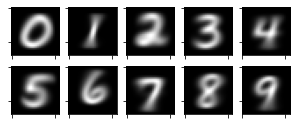
\includegraphics[width=0.7\linewidth]{assets/centroids.png}
		\caption{مراکز خوشه بندی}
	\end{figure}
	می توانیم الگوریتم خوشه بندی را به صورت زیر فرمول بندی کنیم
	\begin{enumerate} 
		\item 
		مرکز ارقام را با استفاده از داده های آموزشی به دست آورید
		\item 
		فاصله هر داده را\footnote{در اینجا منظور فاصله اقلیدسی است.} با مراکز اندازه گیری کنید. داده نامعلوم را به نزدیک ترین خوشه نسبت دهید.
	\end{enumerate}
	با اجرای این الگوریتم توانستیم داده های تست را با دقت ۰۳.۸۲ طبقه بندی کنیم. 
	\pagebreak
	\subsection{ارقام ویژه}
فرض کنید $ \mathbf{A} \in \mathbb{R}^{m \times n} $ ماتریسی باشد که ستون هایش از داده های آموزشی برای یکی از ارقام تشکیل شده. در این صورت ستون های $ \mathbf{A} $ زیرفضایی از $\mathbb{R}^{m} $ را اسپن می کند. انتظار نمی رود که این زیرفضا، زیرفضایی با بعد بالا باشد، چراکه در غیر اینصورت زیرفضا های ارقام متفاوت هم دیگر را می پوشانند و با توجه به خوشه بندی قسمت قبل این امر بعید است. 
هر ستون در $ \mathbf{A} $ یک تصویر را نشان می دهد. از نمایش ضرب خارجی، که در بخش قبل معرفی شد،‌ داریم 
	\begin{center} 
		$ \mathbf{a_j} = \sum_{i=0}^{m} \left(\sigma_i v_{ij}\right) u_i \approx \sum_{i=0}^{k} \left(\sigma_i v_{ij}\right) u_i \approx \sum_{i=0}^{k} \alpha_i u_i$ 
	\end{center} 
	
	پس می توان هر عکس را به صورت تقریب خطی $ u_i $ ها نمایش داد. با توجه به مطالب گفته شده در \hyperref[sec:mat_approx]{تقریب ماتریس} می دانیم که بردار های متناظر با اولین مقدار ویژه اهمیت ویژه ای در کنترل جهت ماتریس داده دارد. در نتیجه انتظار داریم که با رسم $ u_1 $ برداری شبیه به ارقام ماتریس داده داشته باشیم. بعلاوه برای بقیه $ u_i $ ها با بزرگ تر شدن $ i $ از اهمیت $ u $ کاسته می شود. در شکل زیر سه رقم ویژه اول برای سه و شش نمایش داده شده. 
	
	\begin{figure}[h]
		\centering
		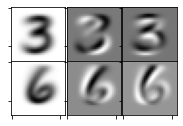
\includegraphics[width=0.3\linewidth]{assets/bases_3_6.png}
		\caption{بردار های ویژه برای اعداد ۳ و ۶}
	\end{figure}
	
	به بردار های ویژه، در اینجا ارقام ویژه\LTRfootnote{eigen digits} نیز گفته می شود. برای دیدن بردار ویژه بیشتر به \hyperref[sec:eigen_digits]{ارقام ویژه} به پیوست مراجعه کنید. 
	
	 \subsection{الگوریتم ارقام ویژه}
برای تقریب هر عکس، $ z $, با استفاده از ارقام ویژه $ u_1, u_2, \ldots, u_k $ باید مسئله مینیمم سازی زیر حل شود
\begin{center} 
	$ min_{\alpha} \vert\vert z - U_k\alpha \vert\vert $ 
\end{center}
که $ \alpha \in \mathbb{R}^k $ بردار ضرایب می باشد. با توجه به متعامد بودن بردار های ویژه می توان گفت $\alpha = U_k^Tz $.

الگوریتم ارقام ویژه را به صورت زیر فرمول بندی می کنیم 
\begin{enumerate}
	\item
	تجزیه مقادیر تکین را برای هر رقم با استفاده از داده آموزش به دست می آوریم. 
	\item 
	به تعداد مناسب\footnote{راجب تعداد مناسب در ادامه بحث خواهد شد}  ارقام ویژه از ستون های ماتریس $ \mathbf{U} $  انتخاب می کنیم. 
	\item 
	هر عکس در داده های تست را با استفاده از پایه های ارقام ویژه برای ارقام مختلف تقریب می زنیم. 
	\item
	عکس را در دسته ای قرار می دهیم که بهترین تقریب، کمترین خطا، را داشته باشد.
\end{enumerate}
	این الگوریتم مربوط به روش SIMCA \cite{simca} است.
	\pagebreak

		نشان می دهیم الگوریتم بالا می تواند نتایج معقولی را برگرداند. شکل زیر مقدار باقی مانده داده آموزشی برای اعداد ۳ و ۷ را با استفاده از ۱۰ رقم ویژه اول در ایه های مختلف نشان می دهد. \\[5pt]
 
 	 \begin{figure}[h]
 		\centering
 		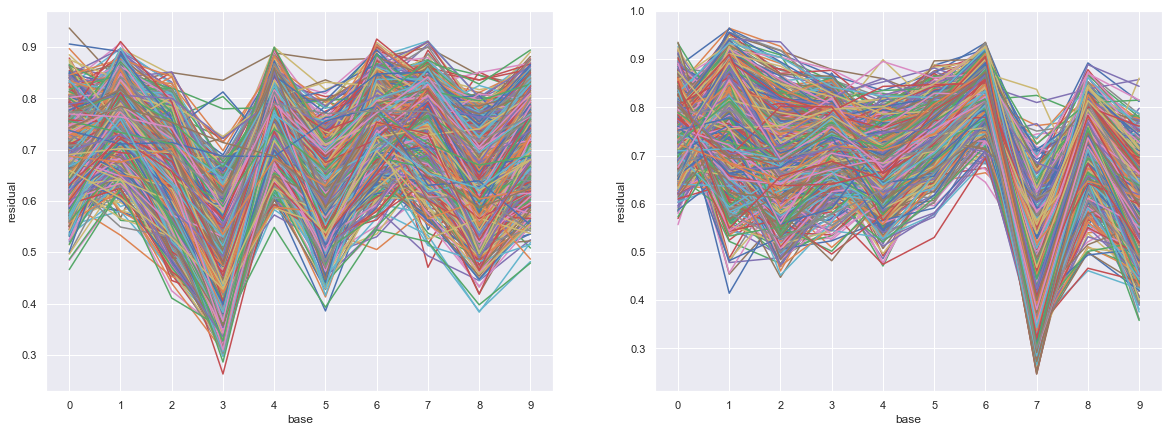
\includegraphics[width=\linewidth]{assets/3_7_bases.png} \\[10pt]
 		\caption{خطا در پایه های مختلف}
 	\end{figure}
 	در شکل سمت چپ می توان دید که مقدار خطا در پایه ۳ از بقیه پایه ها کمتر است و در نتیجه می توان اعداد را به عدد ۳ نسبت داد. همچنین می توان دید خطا برای اعداد ۳ در پایه ۵ هم مقدار کمتری نسبت به پایه های دگر دارد که بدلیل تشابه عدد ۳ و ۵ است.\\[5pt]
 	با توحه به شکل قبل می توان هر عدد را در پایه های دگر هم تقریب زد. \\
 	 
 	\begin{figure}[h]
 		\centering
 		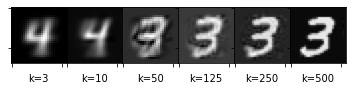
\includegraphics[width=\linewidth]{assets/4_with_3.png} \\[10pt]
 		\caption{تقریب بردار با پایه های متفاوت}
 	\end{figure}
 با اینکه خطای باقی مانده برای عدد ۳ در پایه چهار بالاست،‌اما پایه های چهار توانستند به خوبی ۳ را تقریب بزنند! 
 	
 	\pagebreak
 	بدیهی است که هر چه مقدار $ k $ بیشتر باشد تقریب دقیق تری از داده های آموزش خواهیم داشت.
 	
 	\begin{figure}[h]
 		\centering
 		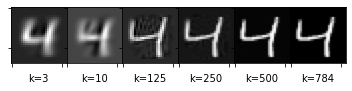
\includegraphics[width=0.8\linewidth]{assets/more_bases_better.png}
 		\caption{تقریب بردار برای مقادیر مختلف k}
 	\end{figure}
 	
 	دو رقم آخر تقریبا غیر قابل تمایز هستند. با ۵۰۰ مقدار ویژه به خوبی توانستیم عکس را تقریب بزنیم. در نتیجه میتوان به جای ذخیره فرم اصلی ماتریس، فرم ناقص را ذخیره کرد.
 	هر چه $ k $ بزرگتر باشد تقریب دقیق تری از عکس داریم. اما تمایل داریم $ k $ را تا جایی که می توانیم کوچک کنیم. 
 	می توان با استفاده از واریانس توضیحی \LTRfootnote{explained variance} مقدار دقت تقریب برای مقادیر مختلف $ k $ را به دست آورد. واریانس توضیحی به صورت زیر تعریف می شود.\\[5pt]
 	\begin{center}
 		$ \mbox{\Large \(%
 			v_k = \frac{\sigma_1 + \sigma_2 + \ldots + \sigma_k } {\sum_{i=0}^n \sigma_i} \) } $ 
 		\\[20pt]	
 	\end{center}
 	
 	در شکل زیر واریانس توضیحی و مقادیر ویژه را برای عدد چهار رسم کرده ایم. همانطور که دیده می شود بردار های ویژه ۶۰۰ به بعد عملا نویز هستند و چیز جدیدی به تقریب اضافه نمی کنند. \\[5pt]
 	\begin{figure}[h]
 		\centering
 		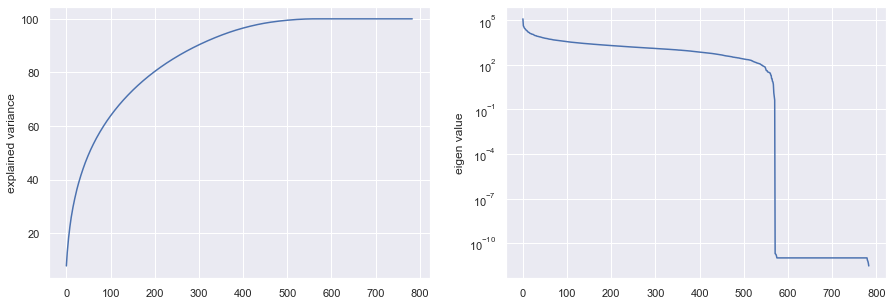
\includegraphics[width=\linewidth]{assets/explained_variance.png}
 		\caption{واریانس توضیحی و مقادیر ویژه}
 	\end{figure}
 	
 	
 	\pagebreak
 	\subsubsection{انتخاب پارامتر k}
 	همانطور که دیدم هر چه مقدار $ k $ بیشتر باشد،‌با استفاده می توان تقریب بهتری از داده های آموزشی داشت. اما آیا چنین چیزی برای داده های تست هم برقرار است؟ 
 	 	 
 	\begin{figure}[h]
 		\centering
 		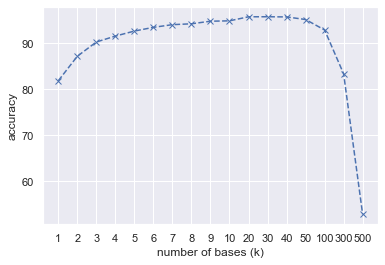
\includegraphics[width=0.8\linewidth]{assets/k_param.png} \\[5pt]
 		\caption{دقت تقریب داده های تست با تعداد پایه های متغیر}
 	\end{figure}
 	شکل بالا نشان می دهد که چنین چیزی نمی تواند برای داده های تست درست باشد. از آنجایی که پایه های مرتبه بالا از اهمیت کمتری برخوردار هستند، انتظار نمی رود که اطلاعات با عمومیت بالایی را در خود ذخیره کرده باشند و بتوان آنها را به داده های تست تعمیم داد. می توان دید برای $ k=5 $ هیچ پیشرفتی نسبت به خوشه بندی قسمت قبل نداشتیم.\\[5pt]
 	 	 	 
 	\begin{figure}[h]
 		\centering
 		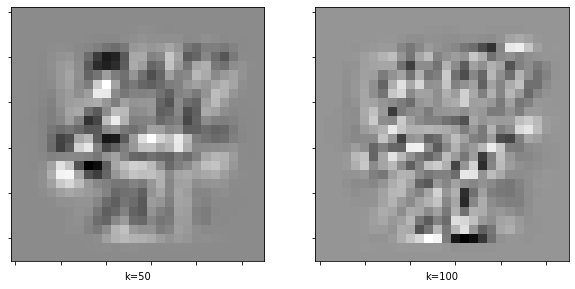
\includegraphics[width=0.6\linewidth]{assets/4_base_k.png}
 		\caption{پایه های ۴ برای مقادیر بالای k}
 	\end{figure}
 	\pagebreak
 	با $ k=30 $ به بهترین دقت رسیدیم. می توان با استفاده از ماتریس درهم ریختگی \LTRfootnote{confusion matrix} نقشه گرمایی\LTRfootnote{heatmap} را برای این مقدار $ k $ رسم کرد. \\
 	\begin{figure}[h]
 		\centering
 		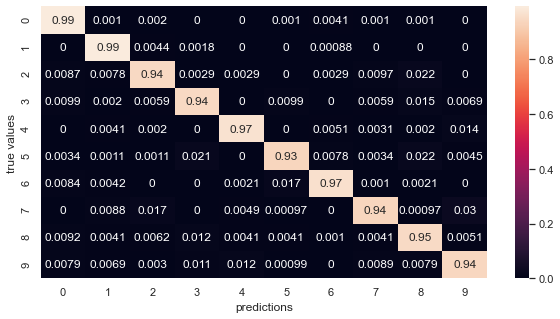
\includegraphics[width=\linewidth]{assets/k=30.png}
 		\caption{ماتریس درهم ریختگی}
 	\end{figure}\\
 	با استفاده از شکل بالا می توان دید چه خطا هایی در مدل وجود دارد. به عنوان مثال رقم ۵ بیشتر ۹ و ۳ اشتباه تشخیص داده شده.\\
 	برای مطالعه بیشتر روش های تبدیل\LTRfootnote{transformation} و استفاده از فاصله تانژانت \LTRfootnote{tangent distance} در دسته بندی ارقام به بخش ۳.۱۰ \cite{matrix_methods} مراجعه کنید.

	
